../cictikz/src/cictikz/data/tex/cictikz_preamble.tex

% The antenna does not radiate - the fields around it do. Left: close
% to the dipole the E field arcs from arm to arm and returns its energy
% to the metal every half cycle. Right: beyond about lambda/2pi the
% field loops close on themselves - displacement current with no metal
% anywhere - and carry power away at c.

\definecolor{echarge}{RGB}{85,155,235}

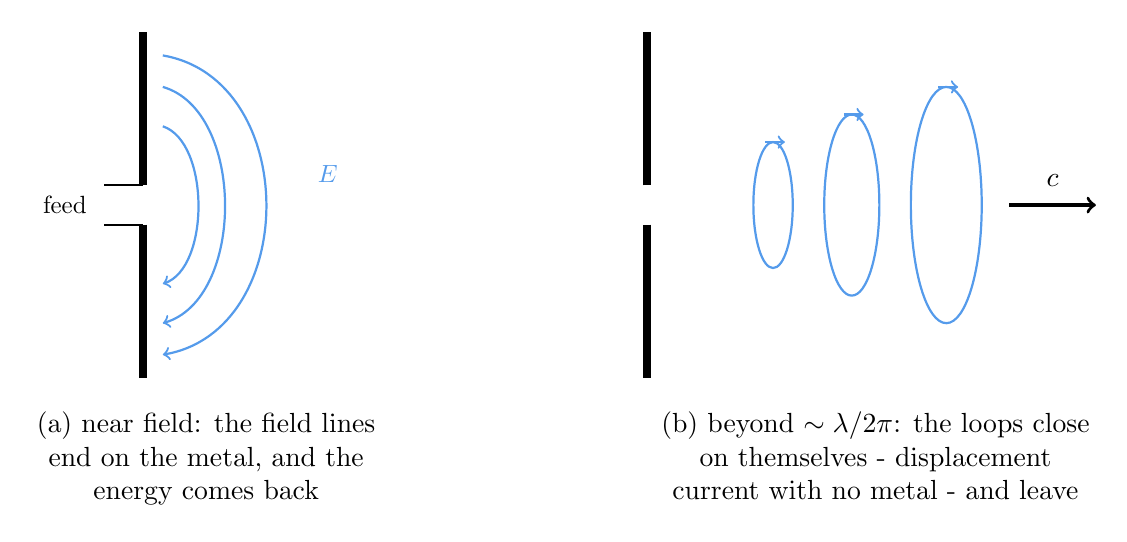
\begin{tikzpicture}[thick]

  % ---------------- (a) near field ----------------
  % the dipole: two arms with a feed gap
  \draw[line width=3pt] (0,0.25) -- (0,2.2);
  \draw[line width=3pt] (0,-0.25) -- (0,-2.2);
  \draw (0,0.25) -- (-0.5,0.25);
  \draw (0,-0.25) -- (-0.5,-0.25);
  \node[anchor=east, scale=0.9] at (-0.6,0) {feed};
  % E field arcs, arm to arm
  \draw[echarge, thick, ->] (0.25,1.5) .. controls (1.3,1.2) and (1.3,-1.2) .. (0.25,-1.5);
  \draw[echarge, thick, ->] (0.25,1.0) .. controls (0.85,0.8) and (0.85,-0.8) .. (0.25,-1.0);
  \draw[echarge, thick, ->] (0.25,1.9) .. controls (2.0,1.6) and (2.0,-1.6) .. (0.25,-1.9);
  \node[echarge, anchor=west, scale=0.9] at (2.1,0.4) {$E$};
  \node[anchor=north, align=center] at (0.8,-2.5)
    {(a) near field: the field lines\\end on the metal, and the\\energy comes back};

  % ---------------- (b) far field ----------------
  \begin{scope}[shift={(6.4,0)}]
    \draw[line width=3pt] (0,0.25) -- (0,2.2);
    \draw[line width=3pt] (0,-0.25) -- (0,-2.2);
    % detached, closed field loops moving right
    \draw[echarge, thick] (1.6,0) ellipse (0.25 and 0.8);
    \draw[echarge, thick, ->] (1.5,0.8) -- (1.75,0.8);
    \draw[echarge, thick] (2.6,0) ellipse (0.35 and 1.15);
    \draw[echarge, thick, ->] (2.5,1.15) -- (2.75,1.15);
    \draw[echarge, thick] (3.8,0) ellipse (0.45 and 1.5);
    \draw[echarge, thick, ->] (3.7,1.5) -- (3.95,1.5);
    \draw[very thick, ->] (4.6,0) -- (5.7,0);
    \node[anchor=south] at (5.15,0.1) {$c$};
    \node[anchor=north, align=center] at (2.9,-2.5)
      {(b) beyond $\sim\lambda/2\pi$: the loops close\\on themselves - displacement\\current with no metal - and leave};
  \end{scope}

\end{tikzpicture}
\end{document}
